\documentclass[11pt]{article}
\usepackage{mystyle}

\title{Synchrotron-$\upmu$CT / MRI spatial registration update}
\author{Scott Trinkle}
\date{Last edited: \today}

\begin{document}

\maketitle

\section{Introduction}

\subsection{Motivation}

Diffusion MRI can be used to calculate metrics that estimate the bulk
orientation of sub-resolution nerve fiber microstructure, such as the
tensor/ellipsoid in diffusion tensor imaging (DTI) or the fiber-orientation
distribution (FOD) in high angular resolution diffusion imaging (HARDI). These
orientation metrics can then be fed into tractography algorithms to estimate the
connectivity of nerve bundles across the brain.

Synchrotron x-ray $\upmu$CT yields images with dramatically higher spatial
resolution. The high resolution allows for the detectability of individual bundles
of myelinated axons. The orientation of these bundles can be estimated using
structure tensor analysis, and the bulk distribution of these orientations
across an arbitrary-sized ROI can be calculated, generating FODs analogous to
those calculated with HARDI imaging. MRI tractography algorithms could be
applied to these $\upmu$CT-generated FOD algorithms and compared to the
segmented nerve bundles themselves for validation. Both of these $\upmu$CT based
connectivity maps could also be compared to tractograms calculated from MRI
data.

Nonlinear spatial registration of the $\upmu$CT and MRI data is needed in order
to perform quantitative, voxel-wise comparison of any of these parameter maps
(FODs, tractograms, or segmented axons bundles). The lower resolution of the MRI
dataset (150~$\upmu$m isotropic vs. 1.2~$\upmu$m isotropic for $\upmu$CT)
provides a challenge to this spatial registration task. The full-resolution
$\upmu$CT dataset is needed to accurately ``ground-truth'' many of these
metrics, but the low resolution of the MRI dataset puts a limit on the feasible
scale of quantitative validation. Additionally, the large size of the $\upmu$CT
dataset poses a significant computational challenge for existing registration
packages / algorithms.

\subsection{Diffusion MRI Validation Literature Review (focus on registration methods)}
Many groups have done studies validating diffusion MRI methods with both
histology \cite{Schilling2016, Schilling2018, Seehaus2015} and polarized light
imaging (PLI) \cite{Mollink2017}.

Mollink et al. \cite{Mollink2017} compared two-dimensional dispersion and
orientation metrics from diffusion MRI (400~$\upmu$m isotropic resolution),
histology ($0.28\times0.28\times6$~$\upmu$m resolution) and PLI
($4\times4\times60$~$\upmu$m resolution) in human brain samples. They calculated
2D deformable transforms using the Modality Independent Neighborhood Descriptor
(MIND) algorithm \cite{Heinrich2012}, which emphasizes local rather than global
similarity. Their input images were the mean diffusivity map from the diffusion
MRI image, the $I_0$ map for PLI and the grayscale stained image for histology.
The calculated deformation fields were applied to the 2D FOD maps, which were
then reoriented using the preservation of principal directions strategy
\cite{Alexander2001}, in which a local affine transformation is computed for
each point in the deformation field and used to reorient the FODs. The success
of the registration was assessed by measuring the distances between manually
identified landmarks. In some regions, they claim accuracy to within 400~$\upmu$m
(i.e., one MRI voxel).

Most groups that have studied 3D \cite{Schilling2016, Schilling2018} and 2D
\cite{Seehaus2015} FOD validation use an MRI/histology registration methodology
published by Choe et al. \cite{Choe2011} at Vanderbilt. The data acquisition protocol is as
follows:
\begin{enumerate}
\item Diffusion MRI is acquired at \textapprox 300-400~$\upmu$m
\item The sample is sectioned at 50-80~$\upmu$m. The block face
  is photographed every 2-3 slices. These photographs are
  stitched together to create a ``block face volume'' with
  through-plane resolution of 150-160~$\upmu$m.
  \begin{itemize}
  \item Choe \cite{Choe2011} recommends downsampling the axial resolution of
    this block face volume, for isotropic voxels of 150-160~$\upmu$m. 
  \end{itemize}
\item A 2D histological montage is acquired with 600-900 tiles for each slice,
  with nominal resolution of 0.80~$\upmu$m. These tiles are stitched together
  with Zeiss software.
\item The Anderson group \cite{Schilling2016, Schilling2018} then identifies a
  number of ROI within each slice to acquire a high-resolution 3D confocal
  subvolume with nominal resolution of $0.18\times0.18\times0.42$~$\upmu$m over
  a $900\times900$~$\upmu$m field of view (equivalent to nine MRI voxels).
  The structure tensor FODs are calculated from these volumes. 
\end{enumerate}

After a number of processing/deconvolution steps to account for tissue shrinkage,
nonisotropic resolution, etc., the registration pipeline proceeds as follows:
\begin{enumerate}
\item The relevent metrics (tensors/FODs) are calculated in their native spaces. 
\item Each 2D histology montage is registered to its corresponding block face
  image with mutual-information based 2D linear registration and 2D nonlinear
  registration with the adaptive bases algorithm (ABA) \cite{Rohde2003}.
\item The $b=0$ (non diffusion-weighted) MRI image is registered to the block
  face volume with 3D affine registration and nonlinear transform
  calculated with ABA.
\item For the Anderson group, given the location of the 3D confocal ROI within
  the 2D montage, the combined deformation fields from MRI $\rightarrow$ block
  face and block face $\rightarrow$ 2D montage are used to determine the MRI
  signal from the same tissue volume.
  \begin{itemize}
  \item The MRI tensors/FODs are then transformed to histological space and
    reoriented using the preservation of principal directions approach
    \cite{Alexander2001} for tensors, or the method developed by Hong et
    al. \cite{Hong2009} for FODs.
  \end{itemize}
\end{enumerate}

Choe et al. validated this methodology by measuring the distance between 291
anatomic landmarks manually identified in both images, with mean accuracies
within one MRI voxel (\textapprox 300~$\upmu$m).

Important to note is that with this method, the MRI is transformed to the
histological space, and the structure tensor FODs from histology are calculated
using MRI-voxel-sized ROI. Thus, in these studies, there is no resampling or
interpolation of the final FODs from either modality. The papers do not address
the multi-scale nature of their registrations from MRI $\rightarrow$ block face
or block face $\rightarrow$ 2D montage. 

\subsection{Application to $\upmu$CT validation study}

This methodology can be adapted for the purposes of comparing FODs calculated
from $\upmu$CT and MRI data. In this case, the higher-resolution (50 $\upmu$m
structural) MRI data can take the place of the intermediate ``block face volume,''
but all comparisons should be performed at the diffusion MRI scale. For FOD
validation, the proposed pipeline is:

\begin{enumerate}
\item Calculate FODs from both datasets using their native
  resolutions. Structure tensor orientations will be calculated with full x-ray
  resolution, but the FODs will be binned over 150 $\upmu$m isotropic ROI.
\item Downsample the $\upmu$CT data and structural MRI data to the diffusion MRI resolution.
\item Calculate the linear and nonlinear $\upmu$CT $\rightarrow$ structural-MRI
  and linear structural-MRI $\rightarrow$ diffusion-MRI spatial transformations.\footnote{Like Choe et al. and the Anderson group, we could assess registration accuracy
    using the distance between manually identified landmarks. We could either do this
    ourselves or find a mouse brain anatomist...}
\item Apply these transformations to the $\upmu$CT FODs (already binned at
  diffusion MRI resolution) to get them into the diffusion MRI space
\item Reorient the FODs appropriately using the methods described in \cite{Alexander2001, Hong2009}.
\item Perform voxel-wise quantitative comparisons (peak angular error, angular
  correlation coefficient, Jensen-Shannon divergence, etc.)
\end{enumerate}

For tractography validation, the same pipeline will apply. If $\upmu$CT
tractography is performed on registered MRI-scale FODs, then no further work is
needed; the same algorithm can be applied to both datasets and any number of
common metrics can be used to evaluate the results \cite{Ning2015,Thomas2014}.
Tractograms can be calculated with subvoxel resolution, so to compare segmented
axon bundles from the $\upmu$CT to tractography results from either dataset, the
difference would appear in Step 2: the $\upmu$CT and structural MRI data will be
downsampled to the tractogram resolution instead of the diffusion MRI data
resolution. New transforms will then be calculated at that resolution and applied to
the segmentation results.

\subsection{Aim}
The original aim of this report was to detail the methods involved in a
different pipeline and to characterize its performance as a function of scale
and interpolation method. This original pipeline involved calculating the
registration at an intermediate resolution achieved by upsampling the MRI
data. I no longer think this is a fair or useful approach. The goal of this
study is to validate commonly used methods of estimating orientation and
connectivity information from diffusion MRI data. The idea of upsampling the MRI
data to an intermediate resolution was to avoid ``wasting'' detail present in
the $\upmu$CT data --- but we never expect diffusion MRI to be able to report
that detail in the first place. Assuming these MRI methods are accurate, we
expect the results to be a downsampled, bulk representation of the ``true''
results calculated from the $\upmu$CT data. Performing the validation at
the native MRI scale will allow us to fairly evaluate that assumption. 

The bulk of an earlier iteration of this report involved a comparison between
two strategies for calculating the transform at an intermediate scale. With the
new proposed pipeline, this question is less relevant --- but for clarity, the
strategies are:

\begin{enumerate}
\item ``Resampled Data'' --- both $\upmu$CT and MRI data are scaled to some common resolution $x$,
  and the transformation is calculated and applied.
\item ``Resampled Transform'' --- the $\upmu$CT data is scaled to the native MRI resolution,
  the transform is calculated, then the transform itself is scaled to some higher resolution $x$
  and applied. 
\end{enumerate}

We expected the ``Resampled Data'' approach to achieve more quantitatively
accurate registrations, but thought the ``Resampled Transform'' approach might
be preferable in situations where it becomes too computationally expensive to
calculate the registration at the desired resolution.

The remainder of this report is unchanged. 

\section{Methods}
\subsection{$\upmu$CT downsampling}
The full 32-bit $\upmu$CT data has a resolution of 1.2~$\upmu$m isotropic.  For
this study, an 8-bit, 4x downsampled (4.8~$\upmu$m isotropic) single-file volume
image was taken as the ``initial'' $\upmu$CT data. This was the highest
resolution version of the $\upmu$CT data that existed as a single file of
manageable size. This data was then downsampled to voxel sizes of 15, 20, 25,
40, 50, 60, 75, 100, and 150~$\upmu$m isotropic using bicubic interpolation
in ImageJ.

\subsection{MRI Resampling}
There are two separate MRI images: a 150~$\upmu$m isotropic image with 30
diffusion-weighting directions, and a 50~$\upmu$m isotropic T$_2$-weighted (?)
structural image. All registrations were calculated using the structural image,
since it was assumed that its higher resolution would lead to better
performance. There is a known affine transformation between these two images
that can be applied to metrics calculated from the diffusion image in the
future.

A mask of the structural image was calculated using a median-otsu thresholding
method in the
\href{http://nipy.org/dipy/examples_built/brain_extraction_dwi.html#example-brain-extraction-dwi}{Dipy
  python package} \cite{dipy} and applied to eliminate edge distortions and background
noise.\footnote{This masking was performed for a separate/previous study, but I
  thought it would improve registration performance to have a harder boundary to
  the brain volume compared to the ``feathery'' boundary of the raw data. See
  Figure \ref{fig:mri_mask}.}

\begin{figure}[h]
  \centering
  \begin{subfigure}[b]{0.45\textwidth}
    \centering
    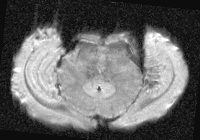
\includegraphics[width=0.8\linewidth]{figs/struct_orig}
    \caption{Raw data}
  \end{subfigure}
  \hspace{1em}
  \begin{subfigure}[b]{0.45\textwidth}
    \centering
    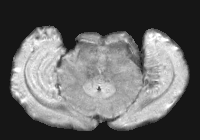
\includegraphics[width=0.8\linewidth]{figs/struct_masked}
    \caption{Masked data}
  \end{subfigure}
  \captionsetup{width=0.9\textwidth}
  \caption{Comparison of raw and masked structural MRI data. Note the undefined boundary
  in the raw image.}
  \label{fig:mri_mask}
\end{figure}

The masked structural image was then resampled to the same resolutions as the
$\upmu$CT data: 15, 20, 25, 40, 50, 60, 75, 100, and 150~$\upmu$m isotropic,
using bicubic, bilinear and ``no'' interpolation in ImageJ.\footnote{I assume that
  the ``Interpolation: None'' option in ImageJ indicates nearest neighbor interpolation}


\subsection{Diffeomorphic registration}
Diffeomorphic registration was performed for every resolution and interpolation
method using the \href{http://stnava.github.io/ANTs/}{Advanced Normalization
  Tools} (ANTs) software package, a interface for the Insight ToolKit image
registration framework~\cite{itk}. ANTs primarily uses the
\href{https://nifti.nimh.nih.gov}{NIfTI-1} (Neuroimaging Informatics Technology
Initiative) data format for image input/output. All images were converted to
this format and the physical voxel dimensions were manually added to the
metadata.

Both affine and diffeomorphic transformations were calculated using the default
parameters of the \newline\verb|antsRegistrationQuickSyN.sh| script. Details are
available
\href{https://github.com/stnava/ANTsTutorial/blob/master/registration/registration.Rmd#lets-start-out-small-and-use-wrapper-scripts}{here},
but a quick summary is provided below:
\begin{enumerate}
\item A rigid transformation is calculated to align the
  centers of mass of the two images. This is performed in four stages, with
  downsampling factors of 12, 8, 4 and 2, smoothing sigmas of 4, 3, 2 and 1 and
  maximum iteration numbers of 1000, 500, 250 and 100, respectively. The mutual
  information (with 32 bins) is optimized in each stage until successive iterations have a
  difference less than 10$^{-6}$ or until the maximum number of iterations is
  reached.
\item An affine transformation is calculated using the same
  parameters as above.
\item A nonlinear, diffeomorphic transformation field is calculated with the
  competition-winning~\cite{competition} ANTs Symmetric Normalization (SyN)
  algorithm \cite{avants2008}. This is performed in five stages, with
  downsampling factors of 10, 6, 4, 2, and 1, smoothing sigmas of 5, 3, 2, 1 and
  0 and maximum iteration numbers of 100, 100, 70, 50 and 20, respectively. The
  cross correlation metric is optimized with a radius of 4, to the same
  convergence criteria as above.
\end{enumerate}

The output is the composite linear transform (4x4 matrix), transform field
(dimension: $X\times Y\times Z \times 3$ for image dimension
$X\times Y\times Z$), and the final transformed image. For these registrations,
the $\upmu$CT image was taken as the ``moving'' image and transformed to the
``fixed'' structural MRI space. This is to avoid the eventual complication of
performing nonlinear transformations on orientation-encoded diffusion MRI
datasets; however, the diffeomorphic SyN transformation calculated by ANTs is
invertible.

\subsection{Transform resampling}
The transform field calculated at 50~$\upmu$m (native structural MRI resolution) was
resampled to each of the other resolutions using each of the three interpolation
methods. Both the composite linear transformation and the resampled transform field
from the 50~$\upmu$m registration were then applied to each of the $\upmu$CT
datasets.

Accordingly, there were a total of six transform fields calculated at each
resolution: three calculated by the ``Resampled Data'' method and three
by the ``Resampled Transform'' method.

\subsection{Analysis}
The mean squared error (MSE), Pearson product-moment correlation coefficient,
and mutual information (MI) were used to quantify the similarity between various
transformations as well as final transformed images.

For $N$ elements, the MSE was calculated as
\begin{align}
  \text{MSE}(X; Y) = \frac{1}{N}\sum_{n=1}^{N} \left(X_n - Y_n\right)^2,
\end{align}
for objects (images or transforms) $X$ and $Y$. A low MSE indicates high
similarity between objects.

The correlation coefficient was determined by calculating a linear fit between
corresponding values in two objects. In Python, this was implemented with the
\href{https://docs.scipy.org/doc/numpy-1.14.0/reference/generated/numpy.corrcoef.html}{\texttt{corrcoef}}
function in the NumPy library, with flattened arrays of the two objects as
inputs. A correlation coefficient close to 1 indicates high similarity between
objects.

Mutual information is defined as
\begin{align}
  \text{MI}(X; Y) = \sum_{x \in X} \sum_{y \in Y} p(x, y) \text{ln}\left(\frac{p(x,y)}{p(x) p(y)}\right),
\end{align}
where $p(x,y)$ is the joint probability function of $X$ and $Y$, and $p(x)$ and
$p(y)$ are the marginal probabilties of $X$ and $Y$, respectively. A high mutual
information indicates high similarity between objects. The $p(x,y)$ was
implemented using the normalized NumPy
\href{https://docs.scipy.org/doc/numpy-1.14.0/reference/generated/numpy.histogram2d.html}{\texttt{histogram2d}} function with 1024 bins. The marginal probabilities were calculated by summing $p(x,y)$ over each axis (equivalent to calculating two 1024-bin one-dimensional histograms).

\section{Results}
\subsection{Affine Transform}

\begin{figure}[h]
  \centering
  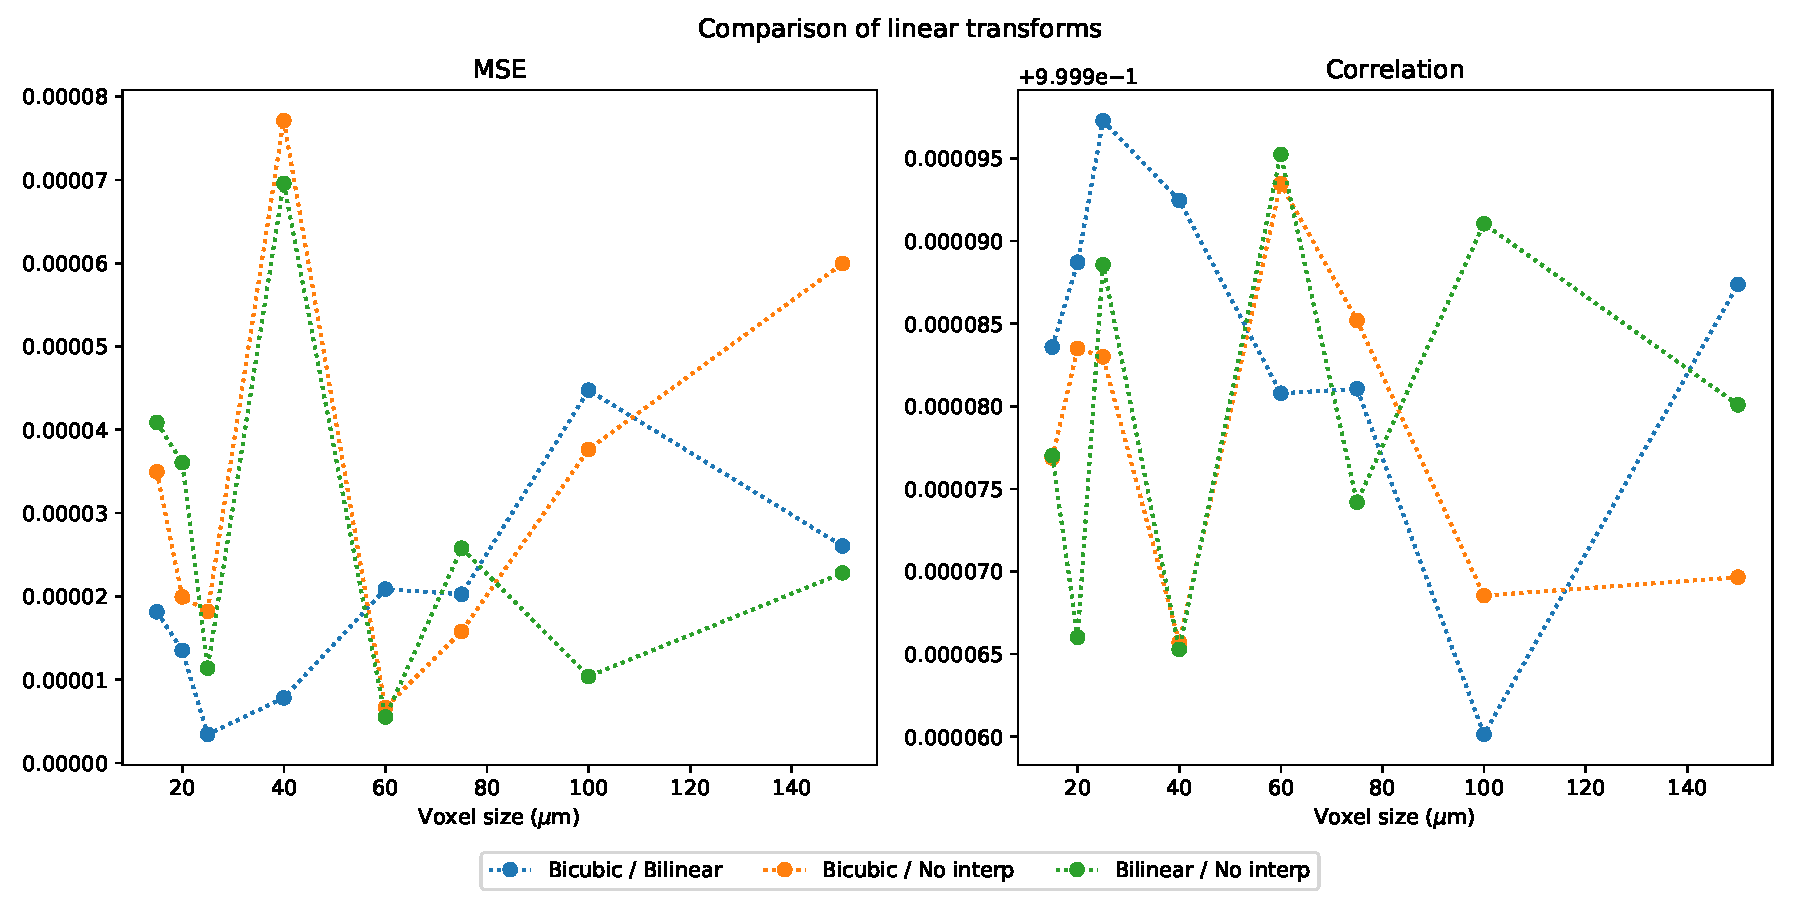
\includegraphics[width=\linewidth]{../results/plots/affine}
  \captionsetup{width=0.95\linewidth}
  \caption{Comparison of linear transform elements. There are no clear patterns
    or trends with respect to resolution or interpolation method.}
  \label{fig:affine}
\end{figure}

Figure~\ref{fig:affine} shows the MSE and correlation of the 12 linear transform
elements as a function of interpolation and resolution. Accordingly, this figure
does not assess the accuracy of the transforms, but their stability across
different interpolation scales and methods.  Overall, the transforms show
extremely good agreement with each other, with very low MSE and high
correlation across all resolutions and interpolation methods. 


\subsection{Transform Field}

\begin{figure}[h]
  \centering
  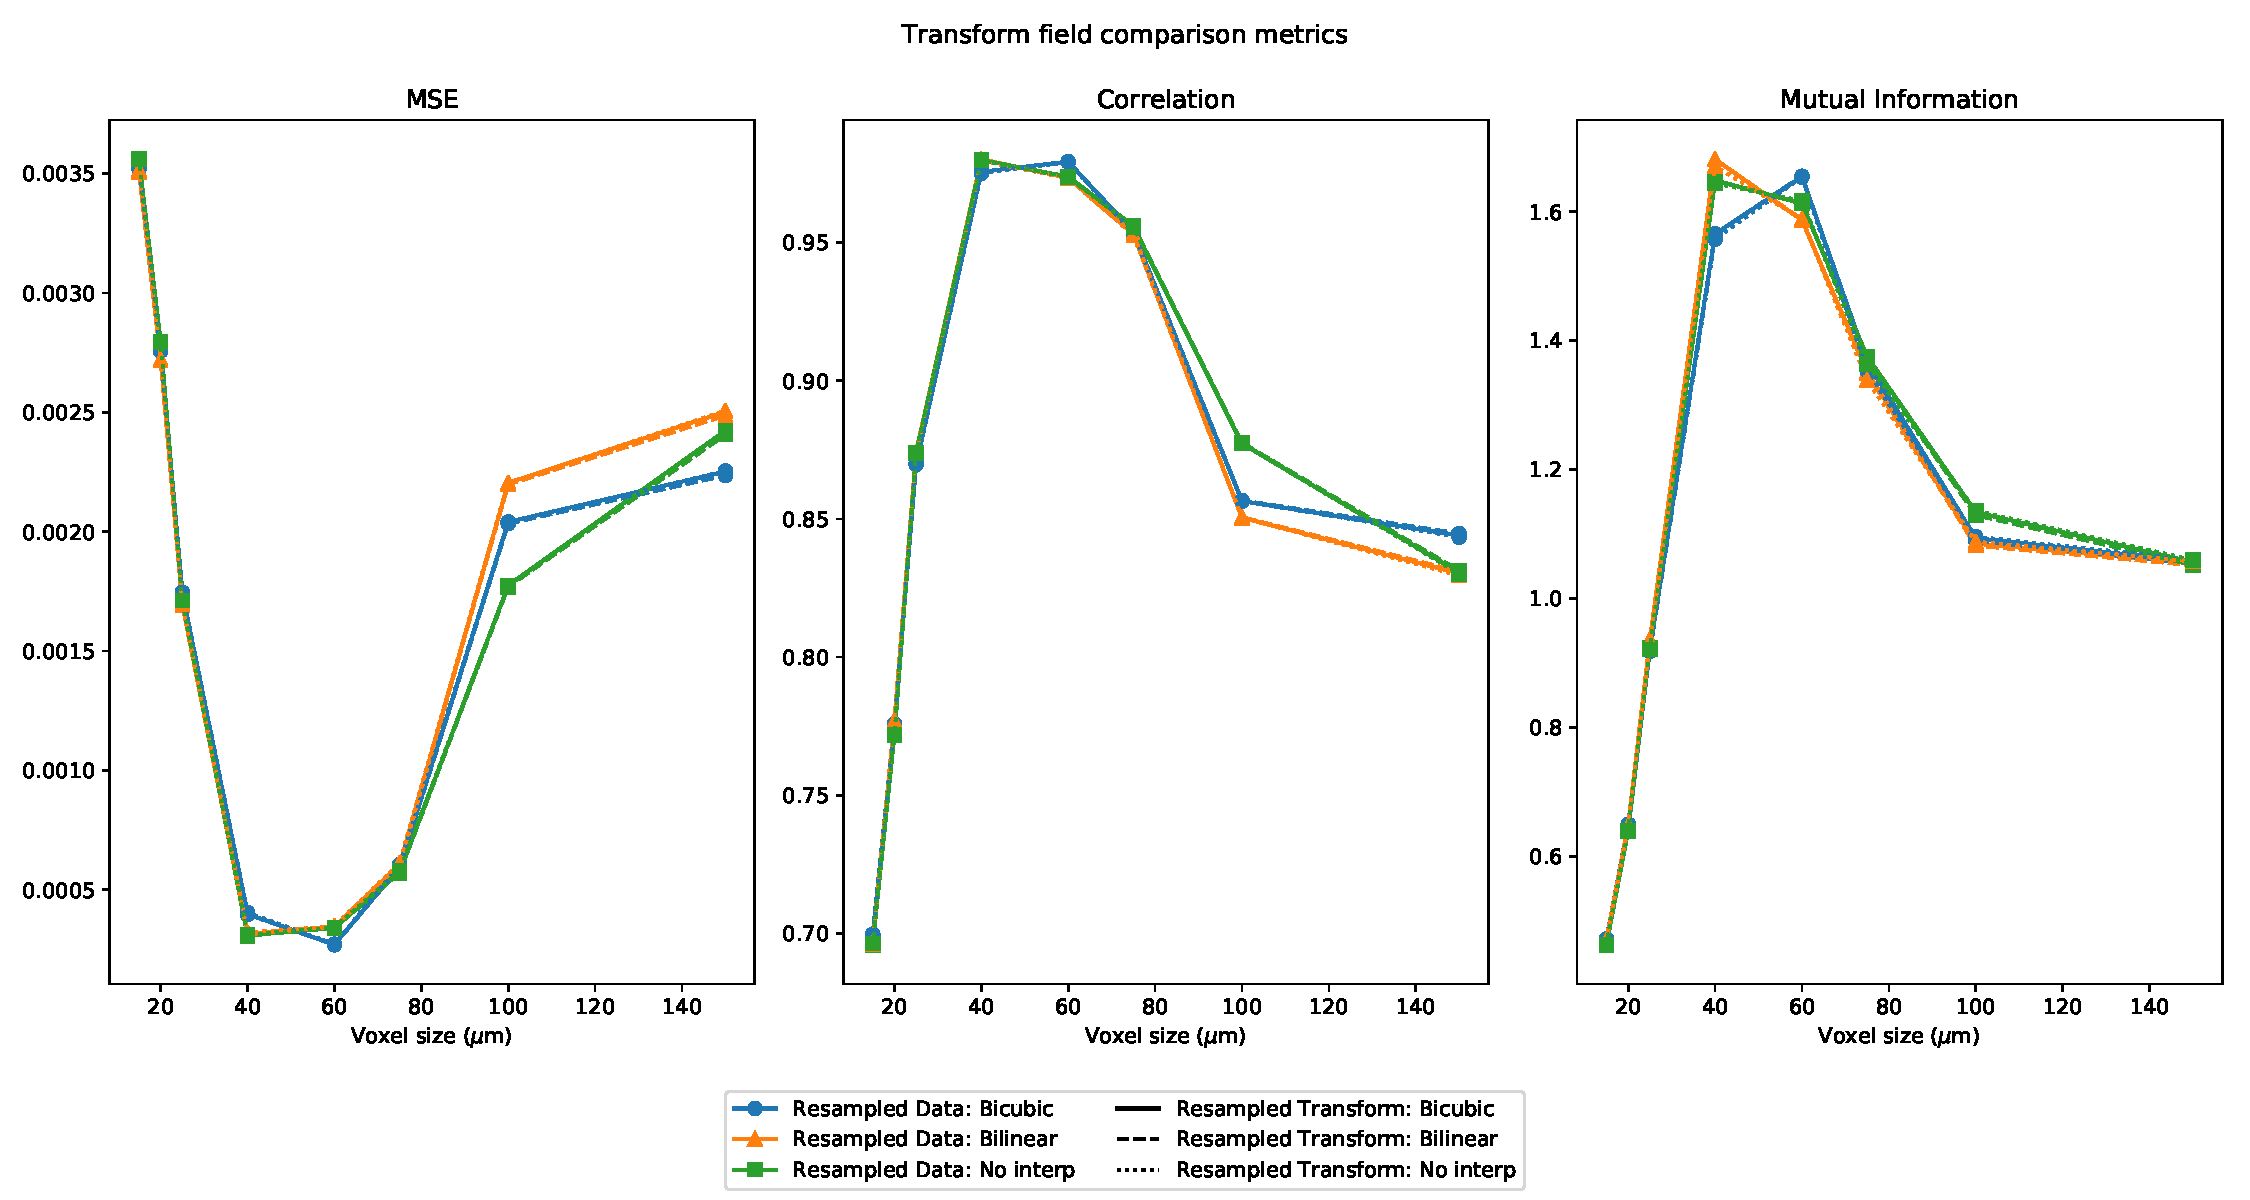
\includegraphics[width=\linewidth]{../results/plots/warp_field}
  \captionsetup{width=0.95\linewidth}
  \caption{Comparison of transform fields calculated from resampled data to
    those calculated at the native resolution and then resampled.}
      \label{fig:warp}
\end{figure}

Figure~\ref{fig:warp} compares the transform fields calculated from resampled
MRI data to those calculated at 50~$\upmu$m and resampled
to the various resolutions. There are nine curves
plotted for each metric: each of the three ``Resampled Transform'' interpolation
methods is compared to each of the three ``Resampled Data'' methods for each
resolution. Line color and marker style indicate the ``Resampled Data''
interpolation method in the comparison, and the line style indicates the
``Resampled Transform'' interpolation method (for example, the solid, orange line with
triangle markers is plotting the comparison between the transform calculated
with bilinear-interpolated MRI data and the bicubic-interpolated transform
originally calculated with native-resolution MRI data).

There are a few notable trends in these plots. First, curves with different line
styles are virtually identical, indicating that the similarity of the transforms
depends much more on the data interpolation method than the transform
interpolation method. In other words: for a given resolution, there is more
variability between transforms calculated \textit{at} that resolution using
differently interpolated data than there is between a single calculated transform
undergoing different interpolations \textit{to} that resolution.

There is also a peak similarity associated with each metric around the native
resolution of 50~$\upmu$m. This leads to the unsurprising result that the
``resampled data'' and ``resampled transform'' approaches are the most similar
near the native resolution at which the resampled transform is calculated. In
other words, as you get further from 50~$\upmu$m resolution, resampling the 50
$\upmu$m transform will yield an increasingly worse estimate of the transform
calculated from resampled data, with very little dependence on interpolation
method. Notably, this effect is more severe at smaller voxel sizes, where there
is much more $\upmu$CT data to utilize when calculating the registration.


\subsection{Registration performance}

\begin{figure}[h]
  \centering
  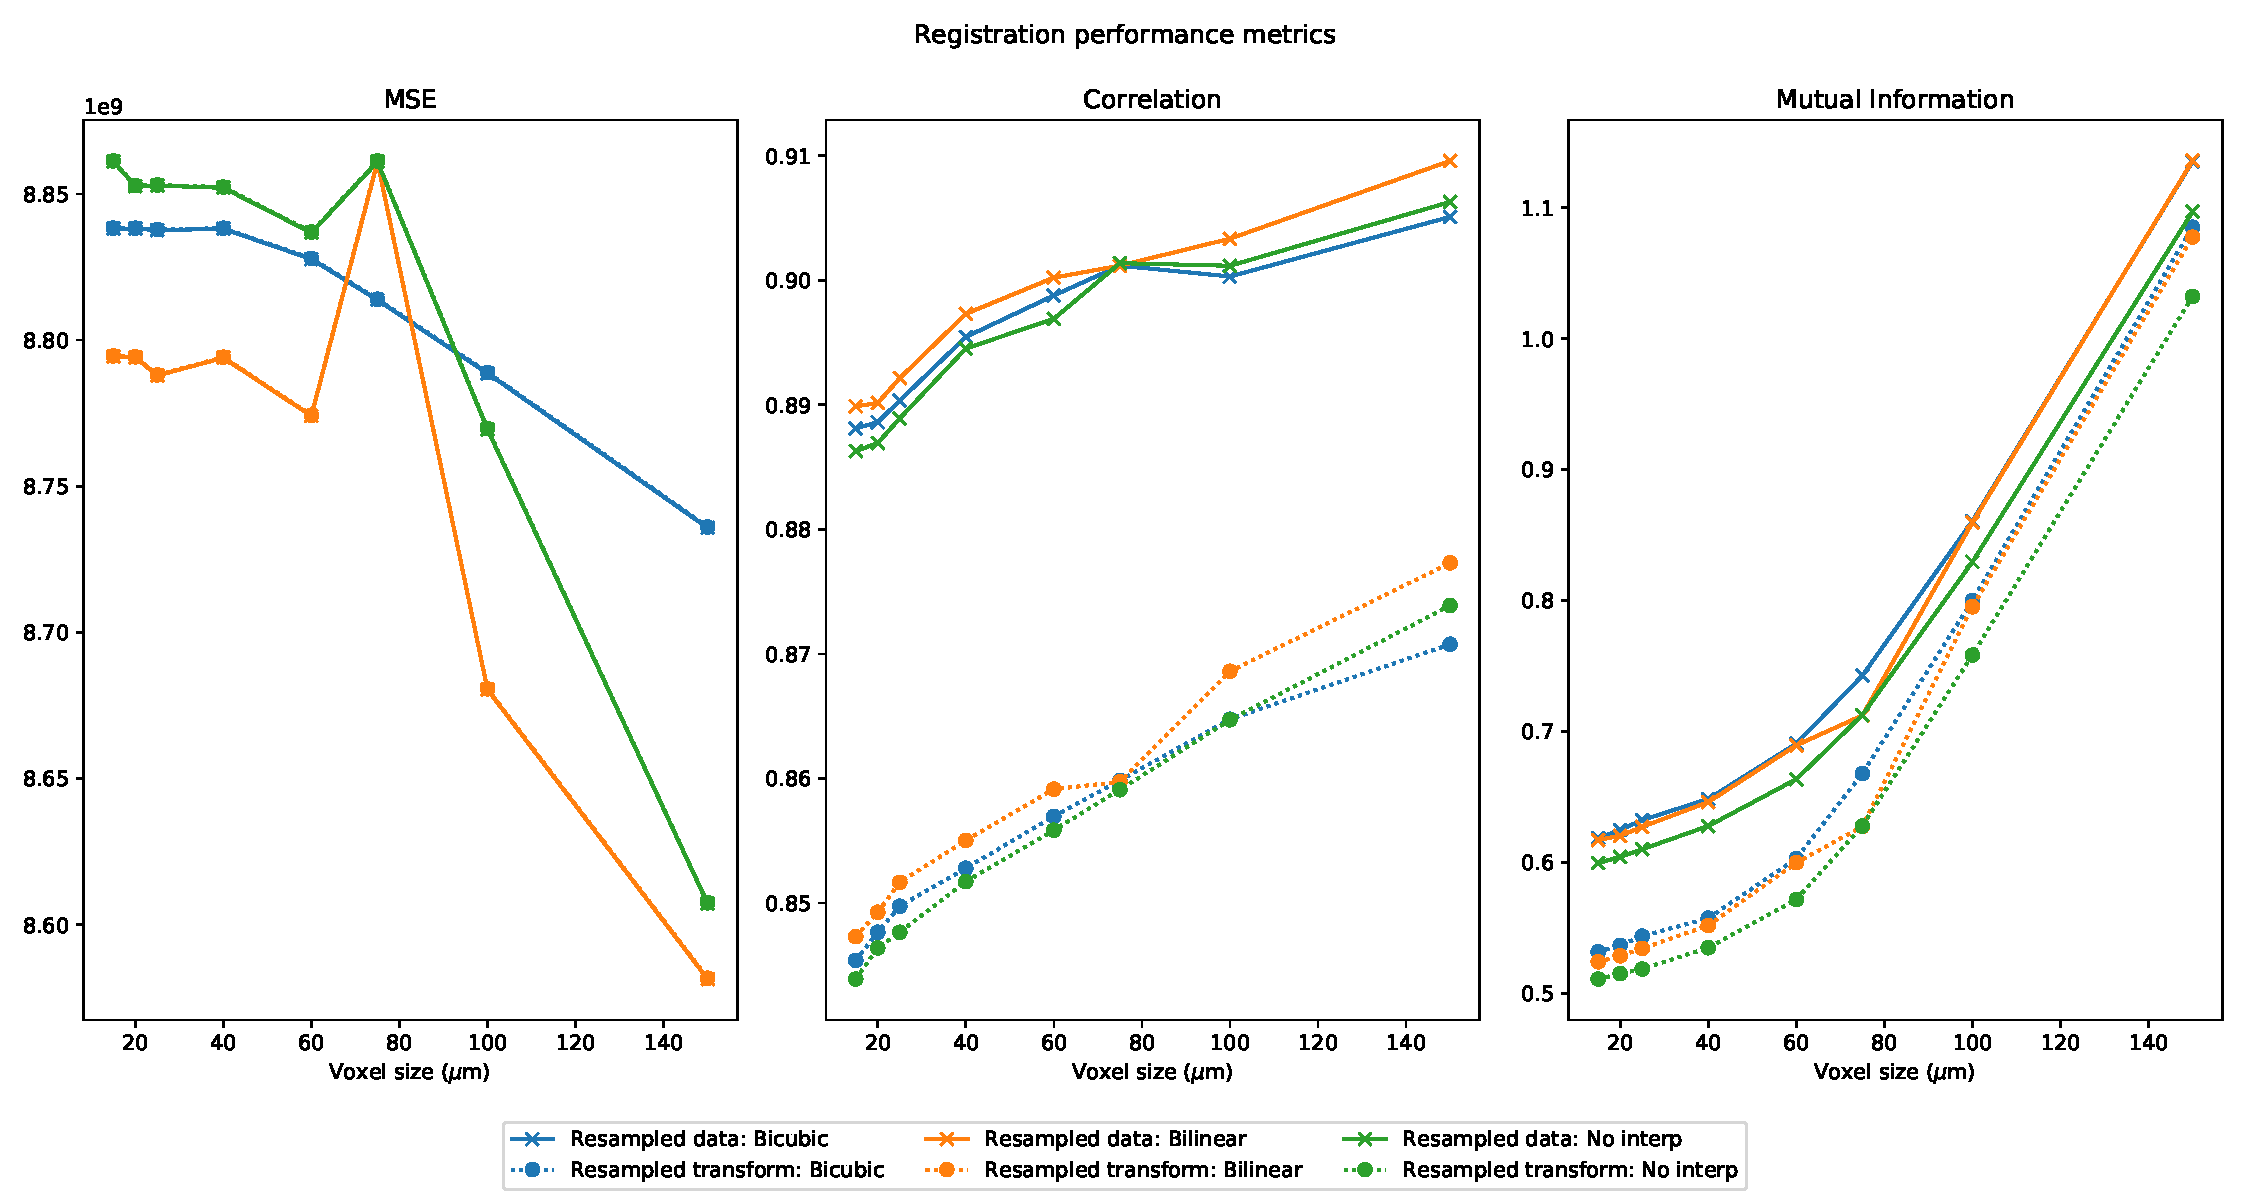
\includegraphics[width=\linewidth]{../results/plots/warped_image}
  \captionsetup{width=0.95\linewidth}
  \caption{Comparison of transformed $\upmu$CT data to MRI from all methods
  of calculating the transform.}
  \label{fig:warped}
\end{figure}

The results of Figure~\ref{fig:warp} do not necessarily have implications on
which of the two methods is preferable, just that they diverge as you move
further from the native resolution. Figure~\ref{fig:warped} plots the similarity
between the interpolated MRI data and the transformed $\upmu$CT data. The line
and marker styles indicate either ``resampled data'' or ``resampled transform''
approaches. The color indicates the interpolation method used in both cases. The
interpolation method used to either calculate or resample the transform that was
applied to the $\upmu$CT data always matched the interpolation method used to
create the MRI data in the comparison.

One immediate concern is the dramatically high MSE value at all resolutions
(note the 1e9 indicator at the top of the axis). This results from the fact that
the input $\upmu$CT data are 8-bit [0,255] integer images, while the input MRI
data are 32-bit images with means of \textapprox 50,000. Since this effect was
common to all registrations/transforms, the relative trend is still noteworthy;
however, notice that it is difficult to visualize the difference between the
``resampled data'' and ``resampled transform'' curves using the MSE metric.

In general, the main trends are as follows:
\begin{itemize}
\item Similarity metrics are ``worse'' at higher resolutions. This is expected:
  at higher resolutions, there is an increase in $\upmu$CT information, but no
  corresponding increase in MRI information. It becomes more and more
  challenging to align small, detailed structures in the $\upmu$CT data when those
  structures are missing entirely in the MRI data.
\item The ``resampled data'' approach (solid lines) yields ``better'' similarity
  metrics for every resolution and interpolation metric. This is expected as
  well: transformations calculated from interpolated data are able to be fine-tuned
  to match the deviations / blurring introduced in interpolation. From the mutual
  information metric, we see that this deviation between the two methods grows larger
  at higher resolutions. 
\item The ``optimal'' interpolation metric depends on resolution and changes
  with different similarity metrics. Generally, bilinear or bicubic
  interpolation perform the best, and no interpolation performs the worst. 
\end{itemize}


\section{Conclusions}
As expected, it is clear that there is a difference between the ``resampled
data'' and ``resampled transform'' approaches. It is not immediately clear
whether or not the results in Figure~\ref{fig:warped} indicate that one method
is preferable to another. Resampling the data before calculating the transform
yields a more quantitatively accurate registration, but the useful information
at any resolution is limited to that of the original image --- interpolating to
a higher resolution cannot generate new information.

This point is illustrated in Figures~\ref{fig:50um} and \ref{fig:15um}.
Figure~\ref{fig:50um} shows the results of a transformation calculated at the
native MRI resolution of 50~$\upmu$m. In Figure~\ref{fig:retrans}, this
``native'' transform is upsampled to 15~$\upmu$m and applied to the $\upmu$CT
data. In contrast, Figure~\ref{fig:redata} shows the transformation calculated
using MRI data upsampled to 15~$\upmu$m (Figure~\ref{fig:mri15}). The
``resampled data'' result is quantiatively more similar to
Figure~\ref{fig:mri15} than the ``resampled transform'' result is, but
Figure~\ref{fig:retrans} appears more realistic and less warped; note the wavy
boundary in Figure~\ref{fig:redata}.

In terms of applying these transformations to calculated metrics (FODs, etc.), I
believe that quantitative registration accuracy will be preferred over
``realistic''-looking images when it comes to voxel-wise comparisons. For this
reason, the ``resampled data'' approach is most likely preferred, provided it is
computationally feasible at the desired scale. We want the registration to
account for the changes introduced by interpolation.

However, we need to think about whether or not we actually have anything to gain
by upsampling the MRI metrics at all, particularly if the final goal is to
validate the MRI techniques used to calculate them. As Figure~\ref{fig:warped}
shows, we only expect the registration performance (and thus, the accuracy of
future metric comparisons) to decrease at higher resolutions: we are not
interested in the ability of \textit{upsampled} diffusion MR to report
connectivity information. It might be best to just perform all
comparisons at the native MRI resolution. 


\begin{figure}[h]
  \centering
  \begin{subfigure}[b]{0.3\textwidth}
    \centering
    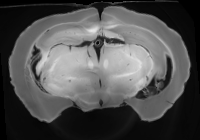
\includegraphics[width=\linewidth]{figs/reg_50umWarped_185}
    \caption{$\upmu$CT}
  \end{subfigure}
  \begin{subfigure}[b]{0.3\textwidth}
    \centering
    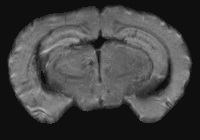
\includegraphics[width=\linewidth]{figs/mri_50um_185}
    \caption{MRI}
  \end{subfigure}
  \hspace{1em}
  \caption{Transformation calculated at native MRI resolution (50~$\upmu$m).}
  \label{fig:50um}
\end{figure}

\begin{figure}[h]
  \begin{subfigure}[b]{0.3\textwidth}
    \centering
    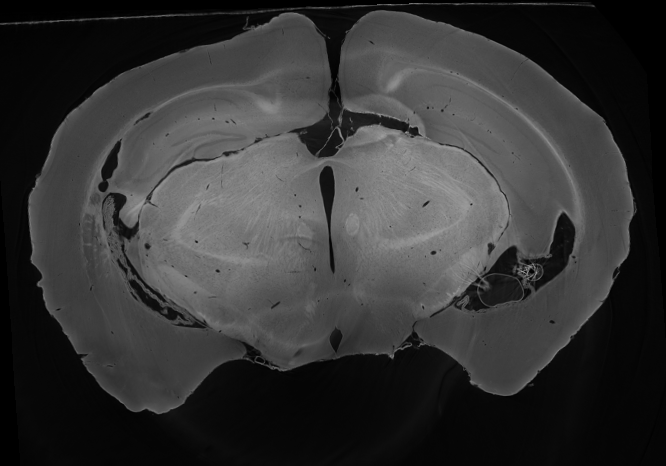
\includegraphics[width=\linewidth]{figs/bilinear_15_sampled_Warped_617}
    \caption{$\upmu$CT: ``resampled transform''}
    \label{fig:retrans}
  \end{subfigure}
  \hspace{1em}
  \begin{subfigure}[b]{0.3\textwidth}
    \centering
    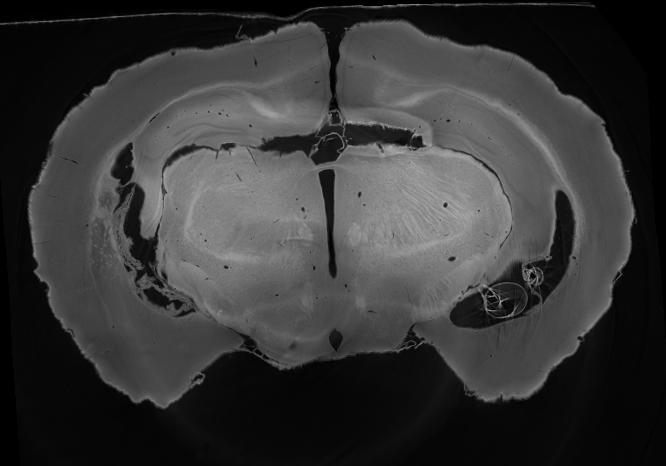
\includegraphics[width=\linewidth]{figs/bilinear_15Warped_617}
    \caption{$\upmu$CT: ``resampled data''}
    \label{fig:redata}
  \end{subfigure}
  \hspace{1em}
    \begin{subfigure}[b]{0.3\textwidth}
    \centering
    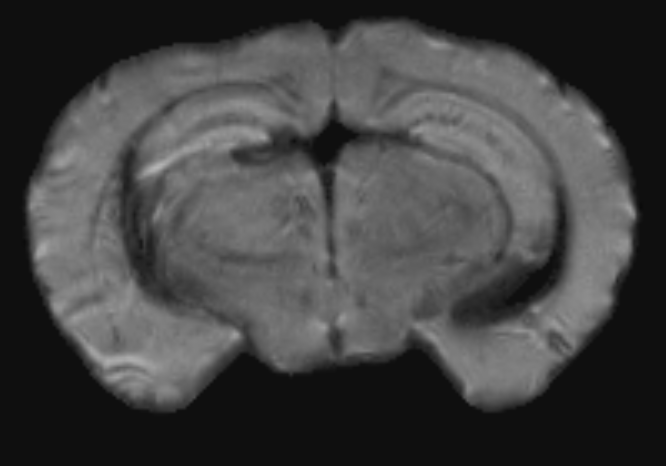
\includegraphics[width=\linewidth]{figs/mri_15um_bilinear_617}
    \caption{MRI}
    \label{fig:mri15}
  \end{subfigure}
  \caption{Transformations calculated with either ``resampled data'' or
    ``resampled transform'' approaches (15~$\upmu$m).}
  \label{fig:15um}
\end{figure}


\section{Future work}
In preparing this report, I came across a few changes I would make to future
registrations. I do not suspect that all of these would have a dramatic effect
on the comparative results presented in Figures~\ref{fig:affine}-\ref{fig:warped},
but they might improve registration accuracy:
\begin{itemize}
\item Mask $\upmu$CT data as well as MRI data
\item Normalize the means of two images before registration
\item Use MI instead of CC as optimization metric in ANTs SyN algorithm
  \begin{itemize}
  \item This metric is commonly preferred for images with different contrast 
  \end{itemize}
\item Let ANTs run to convergence for all registrations
  \begin{itemize}
  \item It reached the max iteration limit for large images, which might play a
    role in the lower reported performance metrics at these scales. 
  \end{itemize}
\end{itemize}

Additionally, I will look closer at the multi-modality, multi-scale registration
literature to see if there are any other insights I have looked over. 

\bibliographystyle{ieeetr}
\bibliography{registrationbib}

\end{document}
